%************************************************
\chapter{Timeline}\label{ch:timeline}
%************************************************

In this chapter I want to update the timeline of my PhD based on the one presented in the initial Research Plan. The project can 
be organized in different stages, which can be the same as the ones presented previously. A Gantt chart showing the different stages 
and their expected duration is also included in Figure \ref{fig:timeline}. 
\begin{itemize}
    \item \textbf{Stage 1: Literature Review and Theoretical Foundations}. This stage will involve an in-depth review of the existing 
    literature on deep generative models (VAEs, Diffusion and Flow Matching), disentanglement representation learning, compositionality, 
    concept bottleneck models, and generative AI for the medical domain. I will also study the theoretical foundations of these 
    topics to identify gaps and opportunities for my research, the key challenges and research questions and define the quantitative and 
    qualitative metrics that I will use to evaluate the performance of my proposed methods. \\
    This stage was planned to be completed in the first 6 months of the PhD, and I have already made significant progress in this area, having 
    reviewed a large number of relevant papers and identified key research questions and challenges that I will address in my research. In the 
    review timeline I have extended the review of the literature to the Q1 of the second year of the PhD, as I will continue to review new papers and 
    developments in the field throughout the duration of the project. 
    \item \textbf{Stage 2: Preliminary experiments}. In this stage, I will conduct preliminary experiments to explore the capabilities 
    and limitations of existing models in terms of disentanglement and compositionality. This will help me to define some baseline models 
    and metrics for evaluating the performance of my proposed methods. This include the reproduction of some key generative models like VAEs,
    Diffusion and Flow Matching, and the implementation of some disentanglement and compositionality metrics. \\
    This stage was planned to be completed between the first 6 and 12 months of the PhD. In the new timeline I have updated it to be between the 
    Q4 of the first year and the Q4 of the second year, with a natural overlap with the previous stage, since I found that implementing and experimenting with the models is a 
    great way to deepen my understanding of the literature and identify gaps and challenges. I have already started conducting several 
    implementations of key models and metrics, where some results were presented in the experiments section.  
    \item \textbf{Stage 3: Method Development and Architectural Innovation}. In this stage, I will develop new methods and architectures for 
    deep generative models that aim to achieve better disentanglement, compositionality, and controllability. This will involve 
    designing novel model architectures, training algorithms, and evaluation metrics to assess the performance of the proposed methods. The idea 
    is to implement modification and extensions of the generative models to enhance their capabilities. \\
    This stage was planned to be completed between the first 12 and 24 months of the PhD. In the new timeline I have modified it to be between the 
    Q3 of the second year and the Q2 of the third year, with a natural overlap with the previous stage, since the insights gained from the preliminary experiments will inform 
    the development of the new methods and architectures. I have already started to develop some preliminary ideas for new methods and architectures, 
    and I plan to continue refining and testing these ideas in the coming months. 
    \item \textbf{Stage 4: Application to the Medical Domain}. In this stage, I will apply the developed methods to the medical domain, 
    specifically focusing on the analysis of medical images focusing on domain-specific challenges like resolution, structure preservation, and clinical 
    realism. Collaborations with medical experts or institutions may be established to assess practical viability and gather expert feedback. Ethical, 
    legal, and data governance considerations will also be reviewed during this phase. In this stage I  will start to work with curated medical image datasets,
    and I will evaluate the performance of the proposed methods in terms of their ability to generate high-quality, clinically relevant images, and to provide 
    insights into the underlying data. \\
    This stage was planned to be completed between the 24 to 30 months of the PhD. In the new timeline I have modified it to be done between the Q2 
    of the third year and the Q1 of the fourth year, with some overlap with the previous stage, since the development of the new methods and architectures 
    will be informed by the specific challenges and requirements of the medical domain. 
    \item \textbf{Stage 5: Evaluation, Validation, and Writing}. In this final stage, I will conduct a comprehensive evaluation of the proposed methods, 
    including both quantitative and qualitative assessments. I will also validate the results through collaborations with domain experts and 
    prepare the findings for publication in peer-reviewed journals and conferences. Additionally, I will write the final thesis document, 
    summarizing the research contributions and outlining future directions for further research in this area. \\
    This stage is planned to be done during the last year of the PhD, between the Q2 and Q4 of the fourth year, with some overlap with the previous stage, 
    since the evaluation and validation of the proposed methods will be an ongoing process throughout the development and application stages. 
\end{itemize}

\begin{figure}[htbp]
    \centering
    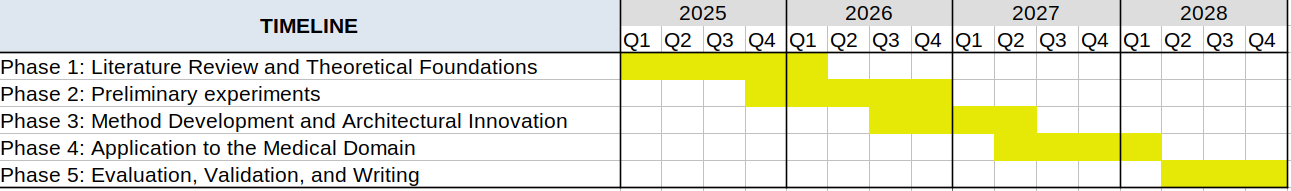
\includegraphics[width=\textwidth]{gfx/timeline/Timeline.png}
    \caption{Updated timeline of the PhD project, showing the different stages and their expected duration.}
    \label{fig:timeline}
\end{figure}


%*****************************************
%*****************************************
%*****************************************
%*****************************************
%*****************************************